\chapter{Aloneness and Freedom}

This chapter follows the fourth Brockwood Park discussion in \emph{The Transformation of Man}, where J. Krishnamurti, in dialogue with David Bohm and David Shainberg, returns to a question left unfinished: why do human beings live in confusion, and why do they not change even when something of that confusion has been seen? There are no validated blackboard frames, equations, or diagram screenshots for this lecture. The mathematical notation below is therefore a disciplined shorthand for relations explicitly developed in the dialogue, not a formal model and not a reconstruction of a board.

The source material is credited to J. Krishnamurti and the Krishnamurti Foundation Trust. This chapter is curated for the \emph{How You Got Happiness?} course by LazyingArt LLC using Video2Book.

\section{The Unanswered Question}

The discussion does not begin with a doctrine of aloneness. It begins with dissatisfaction. The previous day's inquiry had reached the question of whether thought can observe itself, but Krishnamurti says that this was only relevant to the answer. It did not yet answer the human question: why do people live as they do, and why, knowing something of the disorder, do they not change?

That opening rhythm matters. We should not rush to the conclusion. First the dialogue tests the shallow answer: perhaps people like the way they live. But that is immediately seen as inadequate. To change one's conditioning is not merely to exchange a belief. It may mean losing economic stability, losing social place, going against the current, and standing psychologically alone.

The first compact map is therefore only a map:
\begin{equation}
\text{radical change}
\longrightarrow
\text{objective insecurity}
\longrightarrow
\text{standing psychologically alone}.
\end{equation}

It is not yet the whole explanation. It is the first pressure point. If transformation means stepping out of a known stream, the next question is whether human beings can bear aloneness without turning it into isolation.

\subsection{Question \& Answer}

\paragraph{Question.}
Is the fear of transformation merely imaginary?

\paragraph{Answer.}
No. The dialogue is careful here. A person who steps away from the inherited social web may face actual insecurity. The fear is not dismissed as pure fantasy. But the inquiry then separates actual insecurity from the image of being abandoned, unsupported, or cut off from all meaning. That psychological image is where aloneness begins to be mistranslated as isolation.

\section{Security, Group, and the Fear of Standing Alone}

The lecture next examines the pressure to belong. At first this appears as ordinary social togetherness: be with people, be like them, stay inside the accepted pattern. But the dialogue quickly notices that this togetherness is ambiguous. Society may offer a feeling of safety while actually preserving fragmentation.

The first distinction is:
\begin{equation}
\text{being in a group} \neq \text{being truly together}.
\end{equation}

The group may comfort, employ, recognize, and protect. But when it becomes the psychological basis of being, it gives a deeper form of false security. One is no longer merely associated with a group; one feels that without the group one is nowhere.

The lecture's first dependency chain can be written as:
\begin{equation}
\text{group identification}
\longrightarrow
\text{false security}
\longrightarrow
\text{fear of isolation}
\longrightarrow
\text{resistance to change}.
\end{equation}

This notation should be read as transcript-derived shorthand. It is not a causal theory. It is a way to keep the spoken sequence visible: first belonging, then the feeling of safety, then the fear of being outside that safety, then the refusal of radical change.

\begin{figure}
\centering
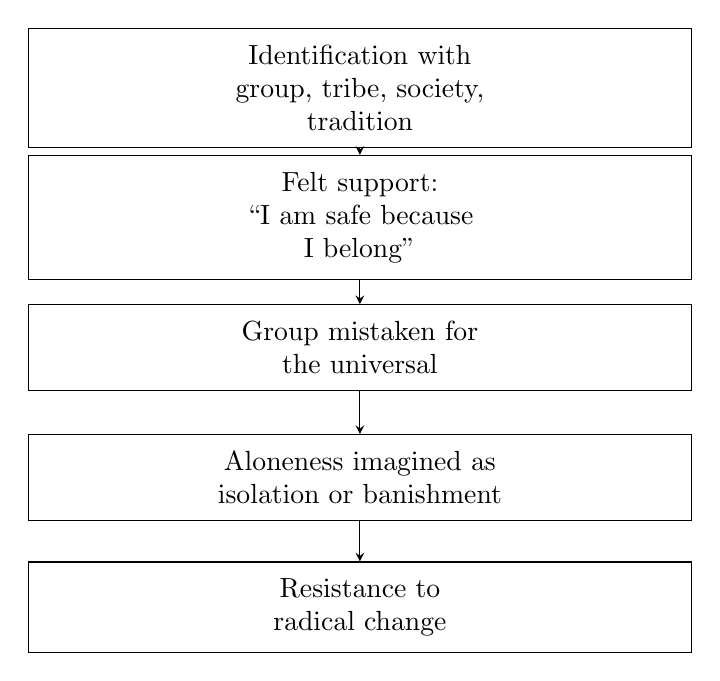
\begin{tikzpicture}[>=stealth, every node/.style={draw, align=center, text width=.66\linewidth, inner sep=6pt}]
\node (a) at (0,0) {Identification with\\group, tribe, society,\\tradition};
\node (b) at (0,-1.65) {Felt support:\\``I am safe because\\I belong''};
\node (c) at (0,-3.30) {Group mistaken for\\the universal};
\node (d) at (0,-4.95) {Aloneness imagined as\\isolation or banishment};
\node (e) at (0,-6.60) {Resistance to\\radical change};
\draw[->] (a) -- (b);
\draw[->] (b) -- (c);
\draw[->] (c) -- (d);
\draw[->] (d) -- (e);
\end{tikzpicture}

Transcript-derived schematic of the first obstacle to change. No validated screenshot supplies a board diagram for this figure.
\end{figure}

\section{The Group as False Universal}

The inquiry now sharpens. It is not enough to say that people dislike being different. The deeper claim is that the group has become the self. The speakers put it plainly: the group is me; I am the group. If I am not in the group, where am I?

That produces a second relation:
\begin{equation}
\text{group} \neq \text{universal},
\qquad
\text{yet the group is felt as universal support}.
\end{equation}

The child may take the tribe, the town, or the immediate social world as the whole. The adult may know abstractly that this is not so, while still feeling that the group is the support of being. This is why banishment carries such psychological force. To be removed from the group is not merely to lose company. It can feel as though one's very orientation has collapsed.

The dialogue therefore revises a familiar philosophical formula. Instead of ``I think, therefore I am,'' the group-bound mind says, in effect:
\begin{equation}
\text{I am in the group}
\longrightarrow
\text{I am}.
\end{equation}

This is the point at which the word ``alone'' becomes dangerous. If the group has been treated as the universal, then to be alone appears to mean being cut off from the universal itself.

\subsection{Question \& Answer}

\paragraph{Question.}
If one is alone, is one cut off from the universal?

\paragraph{Answer.}
No. The lecture answers in the opposite direction. What must be left is the false universal: the group as support of psychological being. Genuine aloneness is not separation from the universal. It begins when false identification with the group is seen, and when the group is no longer taken as the source of one's being.

\section{Aloneness Is Not Isolation}

The distinction now becomes explicit:
\begin{equation}
\text{aloneness} \neq \text{isolation}.
\end{equation}

Isolation is the feared condition: being apart, unsupported, banished, lonely, without anyone to rely on. Aloneness, as the dialogue uses the word, is something else. It means stepping out of the stream of the known: confusion, disorder, sorrow, despair, hope, travail, tradition, and collective psychological knowledge.

So the lecture is not moving from society to private withdrawal. The movement is:
\begin{equation}
\text{group/tradition/known}
\longrightarrow
\text{freedom from the stream}.
\end{equation}

This is why aloneness can be linked to freedom. The point is not that one becomes an isolated individual. The point is that the mind is no longer carrying the burden of psychological tradition as its ground. In that sense, aloneness is not apartness; it is freedom from false dependence.

\begin{table}
\centering
\begin{tabular}{p{.24\linewidth} p{.32\linewidth} p{.34\linewidth}}
\hline
Term & Misread As & Lecture Correction \\
\hline
Group & Universal support & A false universal when taken as the basis of being \\
Isolation & Aloneness & Fearful apartness, banishment, loss of support \\
Aloneness & Loneliness & Freedom from the stream of the known \\
Chaos & A condition to decorate with hope & The actual fact from which inquiry must begin \\
Cosmos & A comforting idea & Order, not projection \\
\hline
\end{tabular}

Pocket-safe table of the chapter's main distinctions.
\end{table}

\section{Chaos, Cosmos, and the Danger of Consolation}

Once aloneness is linked with freedom, the dialogue risks becoming too quick. One might say: if there is freedom, then one is the universe. Krishnamurti interrupts that move sharply. To say ``you are the universe'' while one is confused is dangerous, because it converts disorder into a consoling idea.

The correction is simple and severe:
\begin{equation}
\text{cosmos} = \text{order},
\qquad
\text{chaos} = \text{disorder/confusion}.
\end{equation}

The Greek note in the dialogue is used only to clarify this contrast: cosmos means order; chaos is its opposite. Therefore we cannot begin by asserting inner or universal order while the actual fact is confusion, anxiety, misery, jealousy, and fragmentation. That would be thought projecting a cosmos and taking comfort in the projection.

The disciplined starting point is:
\begin{equation}
\text{actual starting point} = \text{fact of chaos},
\end{equation}
not:
\begin{equation}
\text{actual starting point} = \text{projected cosmos}.
\end{equation}

The lecture's logic is not mystical uplift. It is a guard against premature consolation. If there is disorder, one must begin with disorder. If there is confusion, one must begin with confusion. A projected order is still part of the movement of thought inside disorder.

\subsection{Question \& Answer}

\paragraph{Question.}
Can one say, ``I am the universe,'' while living in confusion?

\paragraph{Answer.}
No. In the dialogue this is called dangerous because it allows thought to invent order while remaining disorderly. Cosmos is order, and order cannot be borrowed as a phrase. One must begin with the fact of what one is. Only then can the word ``alone'' be heard differently: not isolated, but all one, without fragmentation.

\section{Thought, Reality, and the Corporation Called Me}

The lecture then asks again: what prevents radical change? Two reasons have already appeared: fear of isolation and conditioning to accept things as they are. A third appears in language itself. When one says, ``this is all that can be,'' the word ``all'' closes the inquiry. It gives finality to a condition and turns an idea into apparent reality.

Religious and political futures are examined in this light. A religion may project another world; a political system may project a future world. Both may offer a destination made out of the old movement. In that way, even the imagined future can become a subtle way of not being alone.

Then the question becomes direct: why do you not change? The answer is not readily available because the question has not been asked radically. So the inquiry turns to thought. Thought says, ``I cannot change myself,'' and therefore looks for an outside agency: environment, leader, state, God, history. But the same old me remains.

The central relation is:
\begin{equation}
\text{thought} \longrightarrow \text{me},
\qquad
\text{not}
\qquad
\text{me} \longrightarrow \text{thought}.
\end{equation}

The corporation analogy keeps this relation clear. A corporation is treated as though it were an independent reality. It makes money, loses money, pays taxes, owns buildings, and may survive the loss of particular buildings. Yet its reality depends on a whole movement of thought, agreement, law, memory, and recognition.

The ``me'' is treated similarly. Thought creates the me and then attributes thought back to that created center:
\begin{equation}
\text{thought creates me}
\quad \text{but then says} \quad
\text{me creates thought}.
\end{equation}

This is the structure the dialogue calls, in effect, thinking incorporated. The me is not separate from thought. It is the structure of thought, later mistaken for an independent source.

\section{Thought as Movement, Time, and the End of Me}

Now the lecture returns to the question left over from the previous day: does thought see itself in movement? The wording is decisive. It is not, ``I see thought moving,'' because the ``I'' has itself been put together by thought. The question is whether thought is aware of itself as movement.

The late spine of the lecture is:
\begin{align}
\text{thought} &= \text{movement}, \\
\text{movement} &= \text{time}, \\
\text{me} &= \text{time put together by thought}.
\end{align}

Movement means from here to there. Physically, it may be movement from one place to another. Psychologically, it is ``I am this; I must become that.'' That is time as becoming. The me is not an observer outside this movement. The me is continuity generated by the movement.

\subsection{Question \& Answer}

\paragraph{Question.}
Does thought see itself as movement, or does an ``I'' see thought?

\paragraph{Answer.}
The lecture rejects the second formulation. If an ``I'' sees thought, division has already entered: observer here, thought there. But the ``I'' is itself created by thought. The question is whether thought realizes its own movement without inventing a separate center to own the realization.

\paragraph{A worked schematic.}
The dialogue gives a small but important mechanism. Someone says, ``I have a problem; I am suffering.'' That thought carries an implicit ``I.'' Since the ``I'' is felt to be real, the suffering is felt as real in a way that demands more thinking. The next thought says that the problem must be thought about further. Thus the movement sustains the very center that suffers.

As a cautious schematic:
\begin{align}
T_0 &: \quad \text{``I am suffering''}, \\
T_1 &: \quad \text{``Since I am real, this suffering is real''}, \\
T_2 &: \quad \text{``Since it is real, I must think more''}, \\
T_3 &: \quad \text{further thought sustaining the same } I.
\end{align}

Equivalently:
\begin{equation}
\text{thought}
\longrightarrow
\text{image of me}
\longrightarrow
\text{sense of reality}
\longrightarrow
\text{further thought}.
\end{equation}

This is not a formal update rule. It is the dialogue's feedback passage written in note form. Thought gives reality to an image and then responds to that felt reality with more thought. The loop is self-sustaining.

\begin{figure}
\centering
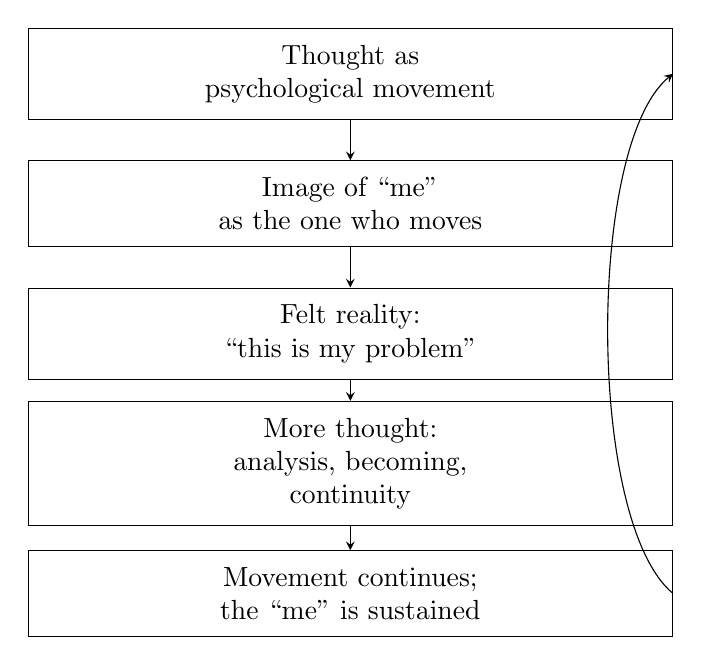
\begin{tikzpicture}[>=stealth, every node/.style={draw, align=center, text width=.64\linewidth, inner sep=6pt}]
\node (a) at (0,0) {Thought as\\psychological movement};
\node (b) at (0,-1.65) {Image of ``me''\\as the one who moves};
\node (c) at (0,-3.30) {Felt reality:\\``this is my problem''};
\node (d) at (0,-4.95) {More thought:\\analysis, becoming,\\continuity};
\node (e) at (0,-6.60) {Movement continues;\\the ``me'' is sustained};
\draw[->] (a) -- (b);
\draw[->] (b) -- (c);
\draw[->] (c) -- (d);
\draw[->] (d) -- (e);
\draw[->] (e.east) .. controls (3.0,-5.7) and (3.0,-.9) .. (a.east);
\end{tikzpicture}

Transcript-derived schematic of the self-sustaining movement of thought. It is an interpretive diagram, not a screenshot reconstruction.
\end{figure}

If that movement stops, the me as psychological continuity has no independent basis. This is why the lecture can say that the ending of movement is felt as death. Not biological death, but the ending now of what thought has put together.

The distinction between psychological and technical thought must be preserved. The lecture does not say that the brain can never again use thought. Technical thought may operate in order. What ends is the movement that creates the me, division, and fear.

\begin{align}
\text{thought as psychological movement}
&\longrightarrow
\text{fragmentary action}, \\
\text{ending of thought-as-movement}
&\longrightarrow
\text{total action}.
\end{align}

The phrase ``total action'' is not a technique. It names the lecture's contrast with action born from division.

\section{Fact, Fear, and Remaining With What Is}

The closing movement is exact. If thought as movement ends, the me ends. The human being hears this as death: not biological death, but the ending of the known self, with its knowledge, possessions, relations as images, and continuity. Krishnamurti then asks how this is received. What takes place in the listener?

The first response is fear or panic. But the dialogue slows down and separates the word from the fact, the image from actuality. Fear is not found in the fact itself. Fear appears when thought makes an abstraction, a picture of ending.

The compact relation is:
\begin{equation}
\text{fact} \longrightarrow \text{no fear}.
\end{equation}

The movement away from fact is:
\begin{equation}
\text{fact}
\longrightarrow
\text{abstraction/image}
\longrightarrow
\text{fear}.
\end{equation}

This is the chapter's sharpest note. It should not be softened into general advice about facing fear. The lecture says something narrower and more demanding: with the actuality of the fact, there is no fear; fear begins when thought moves in and makes an image.

\subsection{Question \& Answer}

\paragraph{Question.}
What happens when the fact is actually seen?

\paragraph{Answer.}
There is no fear. Fear is the idea brought about by abstraction, the picture of ending. When thought comes in, the fact is no longer being stayed with. One is then with imagination, fantasy, or a thought-made reality that feels real.

The dialogue states this strongly: all fear is thought, and all thought is fear or sorrow. We should not turn that into an unqualified formal identity. The immediate context preserves the distinction: technical thought can still function in order. The thought under examination is psychological movement, the movement that creates image, continuity, becoming, and the me.

A cautious notation is therefore:
\begin{equation}
\text{psychological fear}
\subseteq
\text{thought as image-making movement}.
\end{equation}

To remain with the fact is not to explain it, justify it, condemn it, or escape from it. Krishnamurti gives the example of sorrow: can one remain totally with sorrow, not moving into self-pity, method, resistance, or consolation? If thought does not move away, the lecture says, there is extraordinary energy.

\section{Summary}

The lecture unfolds as a return to an unfinished question. Why do human beings not change? The first answer is not psychological abstraction but lived cost: transformation may involve economic insecurity, going against the current, and standing alone.

The inquiry then moves through group security. The group offers support, but when it becomes the basis of being it becomes a false universal. Aloneness is feared because it is confused with isolation, banishment, and loss of orientation. The correction is that aloneness is not isolation; it is freedom from the stream of the known.

The middle of the discussion guards against consolation. Cosmos means order, not a projected idea of order. One must begin with the fact of chaos, not with the assertion that one is already the universe.

The final movement turns to thought itself. Thought creates the me and then treats the me as an independent source. Thought is movement; movement is time; the me is time put together by thought. The ending of that movement is feared as death. But when the fact is actually present, there is no fear. Fear begins with abstraction, image, and the movement away from what is.